\documentclass{amsart}

%\documentclass[10 pt]{amsart}

\usepackage[ocgcolorlinks,linktoc=all]{hyperref}
\hypersetup{citecolor=blue,linkcolor=red}
\usepackage[parfill]{parskip}
\usepackage{graphicx}

%\usepackage{amsthm}
\usepackage{cleveref}
\crefname{lemma}{Lemma}{Lemmata}
\crefname{equation}{equation}{equations}

\newtheorem{theorem}{Theorem}
\newtheorem{lemma}[theorem]{Lemma}
\newtheorem{proposition}[theorem]{Proposition}
\newtheorem{corollary}[theorem]{Corollary}

\newtheorem*{thmA}{Theorem}
\newtheorem*{thmB}{Theorem}
\newtheorem*{rem}{Remark}
\newtheorem*{thmmain}{Theorem}
\newtheorem*{propmain}{Proposition}

\theoremstyle{definition}
\newtheorem{definition}[theorem]{Definition}
\newtheorem{example}[theorem]{Example}
\newtheorem{xca}[theorem]{Exercise}

\theoremstyle{remark}
\newtheorem{remark}[theorem]{Remark}

\numberwithin{equation}{section}

%Symbols
\renewcommand{\~}{\tilde}
\renewcommand{\-}{\bar}
\newcommand{\bs}{\backslash}
\newcommand{\cn}{\colon}
\newcommand{\sub}{\subset}

\newcommand{\N}{\mathbb{N}}
\newcommand{\R}{\mathbb{R}}
\newcommand{\Z}{\mathbb{Z}}
\renewcommand{\S}{\mathbb{S}}
\renewcommand{\H}{\mathbb{H}}
\newcommand{\C}{\mathbb{C}}
\newcommand{\K}{\mathbb{K}}
\newcommand{\Di}{\mathbb{D}}
\newcommand{\B}{\mathbb{B}}
\newcommand{\8}{\infty}

%Greek letters
\renewcommand{\a}{\alpha}
\renewcommand{\b}{\beta}
\newcommand{\g}{\gamma}
\renewcommand{\d}{\delta}
\newcommand{\e}{\epsilon}
\renewcommand{\k}{\kappa}
\renewcommand{\l}{\lambda}
\renewcommand{\o}{\omega}
\renewcommand{\t}{\theta}
\newcommand{\s}{\sigma}
\newcommand{\p}{\varphi}
\newcommand{\z}{\zeta}
\newcommand{\vt}{\vartheta}
\renewcommand{\O}{\Omega}
\newcommand{\D}{\Delta}
\newcommand{\G}{\Gamma}
\newcommand{\T}{\Theta}
\renewcommand{\L}{\Lambda}

%Mathematical operators
\newcommand{\INT}{\int_{\O}}
\newcommand{\DINT}{\int_{\d\O}}
\newcommand{\Int}{\int_{-\infty}^{\infty}}
\newcommand{\del}{\partial}

\newcommand{\inpr}[2]{\left\langle #1,#2 \right\rangle}
\newcommand{\fr}[2]{\frac{#1}{#2}}
\newcommand{\x}{\times}

\DeclareMathOperator{\dive}{div}
\DeclareMathOperator{\id}{id}
\DeclareMathOperator{\pr}{pr}
\DeclareMathOperator{\Diff}{Diff}
\DeclareMathOperator{\supp}{supp}
\DeclareMathOperator{\graph}{graph}
\DeclareMathOperator{\osc}{osc}
\DeclareMathOperator{\const}{const}
\DeclareMathOperator{\dist}{dist}
\DeclareMathOperator{\loc}{loc}

%Environments
\newcommand{\Theo}[3]{\begin{#1}\label{#2} #3 \end{#1}}
\newcommand{\pf}[1]{\begin{proof} #1 \end{proof}}
\newcommand{\eq}[1]{\begin{equation}\begin{alignedat}{2} #1 \end{alignedat}\end{equation}}
\newcommand{\IntEq}[4]{#1&#2#3	 &\quad &\text{in}~#4,}
\newcommand{\BEq}[4]{#1&#2#3	 &\quad &\text{on}~#4}
\newcommand{\br}[1]{\left(#1\right)}



%Logical symbols
\newcommand{\Ra}{\Rightarrow}
\newcommand{\ra}{\rightarrow}
\newcommand{\hra}{\hookrightarrow}
\newcommand{\mt}{\mapsto}

% Aleksandrov Reflection Macros
\DeclareMathOperator{\reflectionvector}{V}
\DeclareMathOperator{\reflectionangle}{\delta}
\newcommand{\reflectionplane}[1][\reflectionvector]{\ensuremath{P_{#1}}}
\newcommand{\reflectionmap}[1][\reflectionvector]{\ensuremath{R_{#1}}}
\newcommand{\reflectionset}[2][\reflectionvector]{\ensuremath{{#2}_{#1}}}
\newcommand{\reflectionhalfspace}[1][\reflectionvector]{\ensuremath{\reflectionset[{#1}]{H}}}
\DeclareMathOperator{\vertvec}{e}
\DeclareMathOperator{\origin}{O}
\DeclareMathOperator{\radialprojection}{\pi}
\DeclareMathOperator{\height}{h}
\DeclareMathOperator{\equator}{E}
\newcommand{\ip}[2]{\ensuremath{\langle{#1},{#2}\rangle}}
\DeclareMathOperator{\intersect}{\cap}
\DeclareMathOperator{\union}{\cup}
\DeclareMathOperator{\nor}{\nu}
\DeclareMathOperator{\basepoint}{p_0}
\DeclareMathOperator{\radialdistance}{r}

%Fonts
\newcommand{\mc}{\mathcal}
\renewcommand{\it}{\textit}
\newcommand{\mrm}{\mathrm}

%Spacing
\newcommand{\hp}{\hphantom}


\parindent 0 pt

\protected\def\ignorethis#1\endignorethis{}
\let\endignorethis\relax
\def\TOCstop{\addtocontents{toc}{\ignorethis}}
\def\TOCstart{\addtocontents{toc}{\endignorethis}}

%\usepackage[left=1in,right=1in,top=1in,bottom=1in]{geometry}
\begin{document}

\title[Ancient solutions to curvature flows in the sphere]
 {On the classification of ancient solutions to curvature flows on the sphere}

\curraddr{}
\email{}
\date{\today}

\dedicatory{}
\subjclass[2010]{}
\keywords{}

\begin{abstract}
We consider the evolution of hypersurfaces on the unit sphere $\mathbb{S}^{n+1}$ by smooth functions of the Weingarten map. We introduce the notion of `quasi-ancient' solutions, which plays a similar role as ancient solutions for flows that do not admit non-trivial ancient solutions. The techniques presented here allow us to prove that any convex, quasi-ancient solution of a curvature flow which satisfies a uniform bound on the second fundamental form backwards in time must be a family of shrinking geodesic spheres. The main tools are geometric, employing the maximum principle, a rigidity result in the sphere and an Aleksandrov reflection argument.
\end{abstract}

\maketitle

\section{Introduction}
\label{sec:intro}

We consider the evolution of convex hypersurfaces $M^n$ by
\eq{\label{eq:CurvFlow}
\partial_tx=-F\nu,~ x:(-T,0)\times M^n\to \S^{n+1},
}
where \(\S^{n+1}\) is equipped with the round metric of constant curvature $1,$ $\nu$ is the outward unit normal to $M_t=x(t,M^n)$ and $F$ is a function of the principal curvatures of $M_t$ satisfying the following properties, which will be assumed throughout the paper without further mentioning.
\begin{ass} \label{F}
Let $\G_{+}=\{(\k_i)\in\R^n\cn \k_i>0~\forall 1\leq i\leq n\}.$ Assume that $F\in C^{\8}(\-\G_{+})$ is 
\begin{enumerate}[(i)]
\item{symmetric}
\item{positive}
\item{strictly monotone, i.e. for all $1\leq i\leq n$ we have
\[\fr{\del F}{\del \k_i}>0.\]}
\end{enumerate}
\end{ass}

We consider \emph{quasi-ancient}, strictly convex solutions of \eqref{eq:CurvFlow}. Here quasi-ancient refers to solutions existing on the same time interval as the maximal flow of geodesic spheres. For many common flows, such as the mean curvature flow \(F(\mathcal{W}) = \text{Trace}(\mathcal{W}) = H\), the maximal flow of geodesic spheres is the infinite time interval \((-\infty, 0)\). However for flows \(F = H^p\) with \(p \in (0,1)\), the maximal time interval is in fact bounded; see \Cref{quasi}.

The following theorem is our main result.
\begin{thm}
Let \(M_t\) be a \emph{quasi-ancient}, strictly convex solution of \eqref{eq:CurvFlow}, where $F$ satisfies \cref{F} and such that
\eq{\limsup_{t\ra -T}\max_{M_t}H<\8.} Then \(M_t\) is a flow of shrinking geodesic spheres.
\end{thm}
In certain situations, such as concave speeds with speed comparable to \(H\), or one-homogeneous convex speeds, the theorem is quite easy to prove, and we offer a short proof in these cases in \Cref{sec:concave_convex_homogeneous}. For instance, this should be compared with the result in \cite[Theorem]{HuiskenSinestrari:05/2014} where a short proof in the case of the mean curvature flow in the sphere may be found. The main idea is to find the correct quantity to which the maximum principle may be applied. In the paper referred to it is the pinching quantity, \((|A|^2 - n H^2)/H^2\) used so often for the mean curvature flow. Here we use \(\mathcal{W}/F\) for concave, mean curvature comparable speeds and the non-collapsing quantity for 1-homogeneous, convex speeds used in \cite{andrews2015Non-collapsing}.

The main thrust of the theorem is that we have very strong rigidity in the sphere, and can prove the result in great generality - \emph{all we require is parabolicity of the flow}. At this level of generality, it is quite difficult to obtain suitable uniform regularity estimates, in particular, Evans-Krylov higher regularity estimates are not known for arbitrary non-linear equations, and hence less direct PDE methods are required. We obtain the theorem by first using the rigidity results of \cite{MakowskiScheuer:/2013} to argue that quasi-ancient solutions with bounded \(H\) must limit to an equator backwards in time. Then the Aleksandrov reflection technique developed in \cite{2015arXiv150802821B,bryanlouie} applies to show the symmetry is preserved under the flow, completing the classification. Let us remark that one may seek other methods of classification, using more PDE theoretic techniques, but they tend to suffer the drawback that they only apply (without modification) to speeds \(F\) that are non-singular and non-degenerate on the equator. The methods we describe here, apply even in the case of \emph{singular or degenerate speeds on the equator}. Very simple examples of such speeds are \(H^p\), which are singular for \(0 < p < 1\) and degenerate for \(p > 1\) whenever \(H = 0\), in particular along the equator. We find that the geometric methods are quite appealing and of interest in their own right, even in cases where PDE methods are applicable, these methods offering a powerful, complementary alternative to direct PDE techniques and supplanting them in cases where such methods are unknown.

One limitation of our method is that at this stage, we assume a bound on the mean curvature \(H\). Although there are certainly solutions emanating from convex polyhedra (and hence with unbounded \(H\)), it is not at all clear to us whether such solutions can be quasi-ancient. In \Cref{quasi}, we give two examples (for non-geometric flows) showing what could go wrong. The first converges to a lune, with unbounded \(H\) and the second converges to an equator, but is not a family of shrinking spheres. Since these examples are not geometric flows, they are not of the type considered here, but they do show that parabolic flows on the sphere may admit ancient solutions that are not a family of shrinking geodesics spheres.

It is also worth comparing the techniques and results here to the Euclidean case. The latter does not exhibit such strong rigidity, and other ancient, convex solutions may occur. Indeed, for the curve shortening flow in the plane, \cite{DaskalopoulosHamiltonSesum:2010} have classified all such solutions as either shrinking circles or the Angenent oval (also known as the paper clip solution) \cite{Angenent:1992}. In higher dimensions, \cite{HuiskenSinestrari:05/2014} and \cite{HaslhoferHershkovits:08/2013} have characterized when ancient, convex mean curvature flows are shrinking spheres, and one would generally expect a greater variety of ancient convex solutions to exist. Convex, ancient solutions are of interest as they arise as rescalings of singularities, cf.~ \cite{HuiskenSinestrari:01/1999}, of mean convex, mean curvature flow, cf.~\cite{HuiskenSinestrari:09/1999, White:10/2002}. Singularity models for mean curvature flow in the sphere have been studied in \cite{Nguyen:2015}, where mean convex singularities with an ambient curvature dependent pinching condition are classified according to a blow-up yielding ancient solutions in Euclidean space, as opposed to the ancient, convex solutions in the sphere studied here.

This paper is laid out as follows: In \Cref{prelim} we establish some notation and basic equations to be used in this paper. In \Cref{quasi}, we introduce the notion of quasi-ancient solutions and establish some facts about such. Then in \Cref{sec:concave_convex_homogeneous} we give a short classification result for concave and 1-homogeneous convex speeds. \Cref{sec:rigidity} contains the rigidity results used to show backwards limits with bounded \(H\) are equators. Then finally in \Cref{sec:reflection}, we use an Aleksandrov reflection technique to complete the classification.

\section*{Acknowledgment}
The authors would like to thank Knut Smoczyk and the Institut f\"{u}r Differentialgeometrie at Leibniz Universität for hosting a research visit where part of this work took place. The first author was a Riemann Fellow at the Riemann Center for Geometry and Physics, Leibniz Universit\"{a}t and was also supported by the EPSRC on a Programme Grant entitled ``Singularities of Geometric Partial Differential Equations'' reference number EP/K00865X/1. The work of the second author was supported by Austrian Science Fund (FWF) Project M1716-N25. All three authors would like to thank Slack.com for providing a wonderful platform for collaboration. 

\section{Preliminaries}\label{prelim}
\label{sec:prelim}
It is well known, compare e.g. \cite[Ch.~2]{Gerhardt:/2006}, that a curvature function as in \cref{F} also can be considered to depend on the Weingarten map,
\[F=F(\mc{W})=F(h^i_j),\]
in case of which the derivatives of the speed \(F\)are written as
\[
F^{i}_{j} = \frac{\partial F}{\partial h^{j}_{i}}.
\]
It is also possible to consider $F$ as a function of the metric and second fundamental form,
\[
F(g, h) = F(g^{ik} h_{kj}),
\]
where we write
\[
F^{ij} = \frac{\partial F}{\partial h_{ij}}, \quad F^{ij,kl} = \fr{\partial^2F}{\partial h_{kl} \partial h_{ij}}.
\]
These derivatives are related by
\[F^{ij}=g^{ik}F^j_k.\]
Let us also define the operator
\[
\Box = F^{ij} \nabla^2_{ij}.
\]
\begin{lemma} \label{lem: basi ev}
The following evolution equations hold:
\eq{
 \label{eq:delt_weingarten_box} 
\partial_t h_i^j &= \Box h_i^j + F^{kl} (h^2)_{kl} h_i^j - (F^{kl}h_{kl} - F) (h^2)_i^j + F^{kl,rs}\nabla_i h_{kl}\nabla^j h_{rs} \\
& \quad +  (F + F^{kl}h_{kl}) \delta_i^j - F^{kl}g_{kl} h_i^j,
}
\eq{\label{eq:delt_speed} \partial_t F = \Box F + FF^{ij}(h^2)_{ij} +  FF^{ij}g_{ij}.}
\end{lemma}

We will occasionally have to work with graphs \(u\) over an equator $E \subset \mathbb{S}^{n+1}$ around a point $e\in\S^{n+1}.$ In geodesic polar coordinates around $e$ the spherical metric takes the form
\eq{\label{SphMetric}d\-s^2=d\rho^2+\vt(\rho)^2\s_{ij}(x)dx^idx^j,}
where $\rho$ is the radial distance to $e,$ $\vt(\rho)=\sin(\rho)$ and $\s$ the round metric on the equator $E\simeq \S^n.$ Hence, if a hypersurface $M$ is given as a graph of a function $u$ over $E$,
\[M=\{(\rho,(x^i))\in \S^{n+1}\cn \rho=u(x),~ x\in E\},\]
a straightforward computation yields the following representation of the Weingarten map in terms of the function $u,$ namely
$$\label{graph h}h^i_j=\fr{\vt'}{v\vt}\d^i_j+\fr{\vt'}{v^3\vt^3}\nabla^iu\nabla_ju-\fr{g^{ik}}{v}\nabla^2_{kj}u,$$
where $v^{-1} = \partial_\rho \cdot \nu.$ Covariant derivatives as well as index raising is performed with respect to $\s_{ij};$ see, for example, \cite[(3.82)]{Scheuer:05/2015}.

A one-parameter family of graphs satisfying the flow \eqref{eq:CurvFlow} is a solution of
\begin{equation}
\label{eq:GraphCurvFlow}
\fr{\del}{\del t}u=-F\br{\fr{\vt'}{v\vt}\d^{i}_{j}+\fr{\vt'}{v^{3}\vt^{3}}\nabla^{i}u\nabla_{j}u-\fr{g^{ik}}{v}\nabla^{2}_{kj}u}v=\Phi(x,u,\nabla u,\nabla^{2}u),
\end{equation}
see \cite[p.~98-99]{Gerhardt:/2006}.

\section{Ancient and quasi-ancient Solutions}\label{quasi}
We are interested in solutions with maximal possible lifetime. To understand this maximal time, we define $T_S$ to be the lifespan of \it{the spherical solution} of \eqref{eq:CurvFlow}. By the spherical solution we mean a family of geodesic spheres shrinking under the flow \eqref{eq:CurvFlow} collapsing to a point at time $t=0$ and existing on the maximal interval \((-T_S, 0)\). For some speeds \(T_S\) is finite.
\begin{lemma}
 Let $p\in(0,1)$ and consider \eqref{eq:CurvFlow} with speed \(F = f^p\) with \(f\) concave and 1-homogeneous. The flow exists only on a finite time interval \((-T_S,0)\) with \(0 < T_S < \infty\), collapses to a point at \(t=0\) and converges to an equator at \(t=-T_S\).
\end{lemma}
\begin{proof}
We may assume that $f(1,\cdots,1)=n.$
Since $F$ is constant on a geodesic sphere, the evolution equation (\ref{lem: basi ev}) for a flow of geodesic spheres yields
$$\fr{d}{dt}f\geq \fr 1n f^{p+2}+ nf^{p},$$
where we used \cite[Lemma~2.2.19, Lemma~2.2.20]{Gerhardt:/2006}.
We obtain finite lifespan forward in time. Integration over some interval $(a,b)$ yield
$$0\leq f^{1-p}(a)\leq f^{1-p}(b)-n(1-p)(b-a).$$
Allowing $a\ra-\8$ gives the finite time existence backwards in time.
\end{proof}
\begin{lemma}
Let $x$ be a convex solution of \eqref{eq:CurvFlow}, defined on the open interval $(-T,0),$ where $0$ is the collapsing time, then $T\leq T_S.$
\end{lemma}
\begin{proof}
Suppose $T>T_S+\e$ for some $\e>0$. Since $M=M_{-T_S-\fr{\e}{2}}$ bounds a convex body $\hat{M}$, it is strictly contained in an open hemisphere due to the classical paper \cite{CarmoWarner:/1970}. Then there exists a geodesic sphere $S$ with $\hat{M}\sub\hat{S}.$ By the avoidance principle, the flow with initial hypersurface $M$ collapses before the spherical flow and thus contradicting $T>T_S$.
\end{proof}
In view of this lemma, the following definition is reasonable.
\begin{defn}
A convex solution of \eqref{eq:CurvFlow} defined on maximal interval $(-T,0)$ is called \it{quasi-ancient}, if $T=T_S$.
\end{defn}
The term ancient is reserved for the situation when \(T_S=\infty\) and by the definition ancient solutions are also quasi-ancient.

For 1-homogeneous and convex speeds, the next proposition gives a bound on mean curvature back wards in time for ancient solutions, using a Harnack inequality. For quasi-ancient solutions, the Harnack inequality does not, in general, give such a bound, since we cannot send \(t \to -\infty\) whenever \(T_S\) is finite. One can envisage backwards limits as convex polyhedra and hence with unbounded \(H\), but it is not clear that these solutions exist on the maximal time interval \((-T_S, 0)\), i.e., they are quasi-ancient solutions. For classification of quasi-ancient solutions, we make the additional assumption that \(H\) is bounded, and defer the question of whether solutions with unbounded \(H\) can exist to a later date.

\begin{prop}
\label{cor:boundedH}
Suppose $F$ is a \(1\)-homogeneous and convex curvature function. Then any convex ancient solution of \eqref{eq:CurvFlow} satisfies
\[\partial_t F-b^{ij}\nabla_i F \nabla_j F \geq 0.\]
Therefore, for all $t\le -1$ we have
$H(\cdot,t)\leq c,$
where $c<\infty$ depends only on $M_{-1}.$
\end{prop}
\begin{proof}
For any $t>s$, the  Harnack estimate of \cite[Theorem 1]{bryan2015harnack} implies that
$$\partial_t F-b^{ij}\nabla_i F\nabla_j F+\frac{1}{2}\frac{F}{t-s}>0.$$
Allowing $s\to-\infty$ proves the first claim. For the second claim, observe that for any 1-homogeneous, convex $F$ we have \[F\ge \frac{F(1,\cdots,1)}{n}H,\]
see \cite[Lemma~2.2.20]{Gerhardt:/2006}. Therefore, ancient solutions satisfy
\[H(\cdot,t)\leq \frac{n}{F(1,\cdots,1)}F(\cdot,t)\leq \frac{n}{F(1,\cdots,1)}F(\cdot,0). \]
\end{proof}
Let us round out this section by looking at some examples of flows for which our techniques do not apply, and the ``undesirable'' behavior ruled out by our assumptions occurs. First, we have a flow that is parabolic, but not geometric, and for which \(H\) becomes unbounded. As mentioned earlier, we do not yet know whether such singular behavior can occur for isotropic, geometric flows.
\begin{example}
We consider a family of convex curves $\gamma_t$ on $\mathbb{S}^2$ that their spherical radial functions evolve by
\[\rho:\mathbb{S}^1\times[0,T)\to \mathbb{R}\]
\begin{equation}\label{eq: angenent oval}
\partial_t\rho(\cdot,t)=-\kappa \frac{\sqrt{\sin^2\rho+\rho_{\theta}^2}}{\sin\rho}\frac{\sin^2\rho+\rho_{\theta}^2}{\tan^2\rho+(\tan\rho)_{\theta}^2}(\cdot,t).
\end{equation}

Here, $\kappa(\cdot,t)$ is the curvature of the curve $\gamma_t$ with the radial function $\rho(\cdot,t).$ 
In polar coordinates we can express the curvature as follows:
\[\kappa=\frac{-\rho_{\theta\theta}\sin\rho+2\rho_\theta^2\cos\rho+\cos\rho\sin^2\rho}{(\sin^2\rho+\rho_{\theta}^2)^{\frac{3}{2}}}.\]
We will show that the gnomonic projection of $\gamma_t$, denoted by $\bar{\gamma}_t$, evolves by the curve shortening flow in $\mathbb{R}^2.$ Write $\bar{\rho}(\cdot,t)$ for the radial function of $\bar{\gamma}_t$. We recall from \cite[p.~8]{besau2014spherical} that
$\bar{\rho}=\tan\rho.$ Using this formula and the expression of $\kappa$ we can write the curvature of $\bar{\gamma}_t$,  $\bar{\kappa}(\cdot,t),$ as follows:
\[\kappa=\left(\frac{\bar{\rho}^2+\bar{\rho}_{\theta}^2}{(1+\bar{\rho}^2)(\sin^2\rho+\rho_{\theta}^2)}\right)^{\frac{3}{2}}\bar{\kappa}=\left(\frac{\bar{\rho}^2+1}{\bar{h}^2+1}\right)^{\frac{3}{2}}\bar{\kappa}.\]
Here $\bar{h}=\frac{\bar{\rho}}{\sqrt{\bar{\rho}^2+\bar{\rho}_{\theta}^2}}$ is the support function of $\bar{\gamma}.$
Therefore, 
\begin{align*}
\partial_t\bar{\rho}&=-\bar{\kappa}(1+\bar{\rho}^2)\left(\frac{\bar{\rho}^2+\bar{\rho}_{\theta}^2}{(1+\bar{\rho}^2)(\sin^2\rho+\rho_{\theta}^2)}\right)^{\frac{3}{2}}\frac{\sqrt{\sin^2\rho+\rho_{\theta}^2}}{\sin\rho}\frac{\sin^2\rho+\rho_{\theta}^2}{\tan^2\rho+(\tan\rho)_{\theta}^2}\\
&=-\bar{\kappa}(1+\bar{\rho}^2)^{\frac{3}{2}}\left(\frac{\bar{\rho}^2+\bar{\rho}_{\theta}^2}{(1+\bar{\rho}^2)(\sin^2\rho+\rho_{\theta}^2)}\right)^{\frac{3}{2}}\frac{\sqrt{\sin^2\rho+\rho_{\theta}^2}}{\bar{\rho}}\frac{\sin^2\rho+\rho_{\theta}^2}{\tan^2\rho+(\tan\rho)_{\theta}^2}\\
&=-\bar{\kappa}\frac{\sqrt{\bar{\rho}^2+\bar{\rho}_{\theta}^2}}{\bar{\rho}}.
\end{align*}
The curve shortening flow in $\mathbb{R}^2$ has non-trivial ancient solutions, the Angenent ovals. Thus, there exists a non-trivial convex ancient solution to flow (\ref{eq: angenent oval}). This ancient solution converges backwards in time to a lune (the intersection of two hemispheres) with a pair of antipodal points at which \(\kappa\) is unbounded.
\end{example}
The second example exhibits a (non-geometric) flow for which the symmetry of the backwards limit is not preserved. That is, the backwards limit is an equator, yet the flow is not by geodesic spheres. 
\begin{example}
We consider a family of convex curves $\gamma_t$ on $\mathbb{S}^2,$ such that their spherical radial functions evolve by
\[\rho:\mathbb{S}^1\times[0,T)\to \mathbb{R}\]
\begin{equation}\label{eq: ellipse}
\partial_t\tan\rho(\cdot,t)=-\kappa^{\frac{1}{3}} \frac{\sqrt{\sin^2\rho+\rho_{\theta}^2}}{\sin\rho}(\cdot,t).
\end{equation}
The gnomonic projection of $\gamma_t$ evolves by the affine normal flow in $\mathbb{R}^2:$ 
\begin{align*}
\partial_t\bar{\rho}&=-\bar{\kappa}^{\frac{1}{3}}\frac{\sqrt{\bar{\rho}^2+\bar{\rho}_{\theta}^2}}{\bar{\rho}}.
\end{align*}
Origin-centered ellipses are ancient solutions to the affine normal flow in $\mathbb{R}^2$ (see, for example, \cite{Ivaki:2016}). Thus, there exists a non-trivial convex ancient solution to the flow (\ref{eq: ellipse}). This ancient solution converges backwards in time to an equator.
\end{example}
\section{Convex, Concave and Homogeneous Speeds}\label{sec:concave_convex_homogeneous}
In this section, we give a quick classification of ancient solutions in two special cases.
\begin{thm}
Let $F$ be $1$-homogeneous, concave and 
$\fr{H}{F}\leq c,$
or let $F$ be $1$-homogeneous and convex. Then any strictly convex ancient solution of the flow \eqref{eq:CurvFlow} with speed $F$ is a family of contracting geodesic spheres.
\end{thm}
\pf{
We first consider the case that $F$ is a concave function. The tensor
$w^j_i=\fr{h^j_i}{F}$
satisfies the evolution equation
\begin{align*}\del_tw^j_i&=\Box w^j_i-2 F^{kl}g_{kl}w^j_i+2\d^j_i+\fr{1}{F}F^{kl,rs}\nabla_ih_{kl}\nabla^jh_{rs}\\
    &\hp{=}-2F^{kl}\nabla_kh^j_i\nabla_l\br{\fr{1}{F}}-2\fr{h^i_j}{F^3}F^{kl}\nabla_k F\nabla_l F.\end{align*}
Due to the concavity of $F$ we have for fixed index $i\cn$
\begin{align*}\del_t\br{w^i_i-\fr{1}{n}}&\leq\Box\br{w^i_i-\fr{1}{n}}-2n\br{w^i_i-\fr{1}{n}}\\
            &\hp{=}-2F^{kl}\nabla_kh^i_i\nabla_l\br{\fr{1}{F}}-2\fr{h^i_j}{F^3}F^{kl}\nabla_k F\nabla_l F.\end{align*}
At a spatial maximum of $w^i_i-\tfrac{1}{n}$ we have
$$0=\nabla_k \br{\fr{h^i_i}{F}}=\fr{\nabla_k h^i_i}{F}+h^i_i\nabla_k\br{\fr{1}{F}}$$
and hence by the maximum principle we obtain the bound
$$w^i_i-\fr 1n\leq c_0e^{-2n t},$$
where $c_0$ is the upper bound for the function on the left-hand side at $t=0.$
Starting the flow at an arbitrary $s<0$ we find
$$\fr{\k_n}{F}\leq \fr 1n+c_se^{-2n (t-s)}.$$
Letting $s\ra-\8,$ we obtain at every time $t<0$ that 
$$\k_n\leq \fr{F}{n}.$$
This is only possible for totally umbilical hypersurfaces, and the result follows since the only closed, totally umbilical hypersurfaces of the sphere are geodesic spheres.

Now suppose that $F$ is a convex and 1-homogeneous function normalized so that $F(1,\cdots,1)=n$. The non-collapsing result of \cite[Thm.~1.2]{andrews2015Non-collapsing} states any ancient solution of the flow with a 1-homogeneous convex speed $F$ satisfies
\[\frac{\kappa_{\min}}{F}(x,t)\geq \frac{1}{n}+C(s)e^{-2n(t-s)},\]
where $|C(s)|\leq \frac{1}{n}+\frac{\kappa_{\min}}{F}(x,s)\leq \frac{1}{n}+\frac{\kappa_{min}}{\frac{F(1,\cdots,1)}{n}H}(x,s)\leq \frac{1}{n}+\frac{1}{F(1,\cdots,1)}.$
Therefore, allowing $s\to-\infty$ yields
\[\frac{\kappa_{\min}}{F}(x,t)\geq \frac{1}{n}.\]
This in turn implies that
\[\kappa_{\min}(x,t)\geq \frac{F}{n}(x,t)\geq \frac{F(1,\cdots,1)}{n}\frac{H}{n}(x,t)\geq \frac{F(1,\cdots,1)}{n} \kappa_{\min}(x,t).\]
On the other hand, since $F(1,\cdots,1)= n,$ we get
\[\kappa_{\min}(x,t)\geq \frac{F}{n}(x,t)\geq \frac{H}{n}(x,t)\geq \kappa_{\min}(x,t).\]
That is, $H\equiv n\kappa_{\min}$; therefore, the flow is by geodesic spheres.
}
\section{Rigidity and Backwards Limit}\label{sec:rigidity}
Now we turn to more general speeds \(F\). The aim of this section is to prove that for a quasi-ancient solution of \eqref{eq:CurvFlow} \it{with bounded mean curvature} for $t\ra -T_S$ the backwards limit of the flow hypersurfaces $M_t$  is an equator. We will use the rigidity result of \cite{MakowskiScheuer:/2013} to achieve this. For convenience, we state this result:
\begin{thm}\label{Rigidity}\textsc{\cite[Theorem 1.1]{MakowskiScheuer:/2013}}
Let $ n\geq 1$ and $\hat{M}\subset \S^{n+1}$ be a weakly convex body in a hemisphere. Let $x_0\in \S^{n+1}$ be such that $\hat{M}$ is contained in the closed hemisphere $\mc{H}(x_0)$ with equator $\mc{S}(x_{0})$. Suppose that $\hat{M}$ satisfies an interior sphere condition at all points $p\in \hat{M} \cap \mc{S}(x_0)$. Then either $\hat{M}$ is equal to $\mc{H}(x_0)$ or $\hat{M}$ is contained in an open hemisphere.
\end{thm}
Here $\hat{M}$ is a weakly convex body in a hemisphere $\mc{H}(x_0),$ if for every two points $p,q\in\hat{M}$ there exists a minimizing geodesic connecting $p$ with $q,$ while being contained in $\hat{M}.$ $\hat{M}$ satisfies an interior sphere condition at $p\in \del\hat{M}$ with radius $R,$ if there exists a geodesic ball $B_R$ with radius $R,$ such that
\[\del B_R\cap\del \hat{M}=\{p\}\quad~\text{and}~B_R\sub\mrm{int}(\hat{M}). \]
Note that the points $p$ in \cref{Rigidity} are automatically boundary points of $\hat{M}.$

The next lemma is the first step in providing the assumptions of \cref{Rigidity}.
\begin{lemma}\label{ISC}
Let $x$ be a quasi-ancient solution of \eqref{eq:CurvFlow} with backwards bounded mean curvature. Then there holds:
\begin{enumerate}
  \item For all $t_0<0$ there exists a uniform radius $R>0,$ such that the enclosed convex bodies $\hat{M}_t,$ $-T_S<t\leq t_0,$ of the flow hypersurfaces $M_t$ satisfy a uniform interior sphere condition with radius $R.$
  \item For every $y_0\in\mrm{int}~\hat{M}_{t_0}$ the hypersurfaces $M_t,$ $-T_S<t\leq t_0,$ can be written as a graph in geodesic polar coordinates around $y_0$ and the corresponding graph functions satisfy uniform $C^2$-estimates.
\end{enumerate}
\end{lemma}
\pf{
Fix an interior point $y_0\in \mrm{int}~\hat{M}_{t_0}.$ Since for a contracting flow the enclosed convex bodies of the flow hypersurfaces are decreasing, they are increasing backwards in time. By the proof of \cite[Lemma~3.9]{MakowskiScheuer:/2013} there exists a closed hemisphere $\mc{H}(x_0),$ such that
$$\hat{M}_t\sub\mc{H}(x_0).$$
In our situation all hypersurfaces $M_t,$ $-T_S<t\leq t_0,$ satisfy
$$B_{\e}(y_0)\sub \mrm{int}~\hat{M}_t$$
and
$$B_{\e}(\hat{y}_0)\sub \hat{M}_t^c$$
with a uniform $\e,$ where $\hat{y}_0$ denotes the antipodal point of $y_0.$
Now we prove the two claims.

(1)~Consider the stereographic projection with $\hat{y}_0$ corresponding to infinity. The image hypersurfaces are then strictly convex hypersurfaces in Euclidean space with uniformly bounded second fundamental form. Blaschke's rolling theorem (see \cite{Blaschke:/1956}) gives the interior sphere condition.\\

(2)~
Write the $M_t$ as graphs in geodesic polar coordinates around $y_0,$
$$M_t=\{(\rho,x^i)\cn \rho=u(t,x^i)\}.$$ 
Due to \eqref{SphMetric}, on the set in which $M_t$ range, the metrics $g_{ij},$ $\-g_{ij}=\sin^2\rho\s_{ij}$ and $\s_{ij}$ are all equivalent.
In view of \cite[Theorem 2.7.10]{Gerhardt:/2006} for all convex hypersurfaces $M_t$, the quantity
$$v^2=1+\-g^{ij}\nabla_iu\nabla_ju$$
is uniformly bounded by a constant which only depends on $\e.$
Hence by the equivalence of norms, $M_t$ are uniformly $C^1$-bounded in the sense that the corresponding functions $u(t,\cdot)$ are uniformly $C^1(\S^n)$-bounded. Recalling equation \eqref{graph h}, due to the curvature estimates we obtain uniform $C^2(\S^n)$-estimates for \(u\).}

\begin{cor}\label{Backlimit}
Let $x$ be a quasi-ancient solution of \eqref{eq:CurvFlow} with backwards bounded mean curvature. Then there exists a unique backwards limiting hypersurface $M_{-T_S}$ and the flow hypersurfaces $M_t$ converge to $M_{-T_S}$ in $C^{1,\b},$ $0<\b<1,$ in the sense that for a common graph representation as in Lemma \ref{ISC} there holds
$$u(t,\cdot)\ra u(-T_S,\cdot)$$
in the norm of $C^{1,\b}(\S^n).$
\end{cor}
\pf{
In view of the point-wise monotonicity of $u(t,\cdot)$ backwards in time, we obtain a point-wise limit. The $C^{1,\b}$-convergence follows from compactness.
}
\begin{thm}
\label{thm:backwardslimit}
The hypersurface $M_{-T_S}$ defined in Corollary \ref{Backlimit} is an equator.
\end{thm}
\pf{
Since the convex bodies $\hat{M_t}$ are increasing backwards in time and due to the uniform convergence of $M_t$ to $M_{-T_S},$ the set
$$\hat{M}_{-T_S}:=\overline{\bigcup_{t<0}\hat{M}_t}$$
is a compact body with
$$\del \hat{M}_{-T_S}=M_{-T_S}.$$
Since $\mrm{int}(\hat{M}_{-T_S})$ is a strictly convex set, it is especially weakly convex in a hemisphere in the sense of \cite[Definition 3.2]{MakowskiScheuer:/2013}. Thus $\hat{M}_{-T_S}$ is a weakly convex body in a hemisphere. The proof of \cite[Lemma 6.1]{MakowskiScheuer:/2013} can literally be applied to show that $\hat{M}_{-T_S}$ satisfies a uniform interior sphere condition as well.
We can apply \cite[Theorem 1.1]{MakowskiScheuer:/2013} and obtain that $\hat{M}_{-T_S}$ is either strictly contained in an open hemisphere or is equal to a closed hemisphere. The first alternative is not possible since the solution is quasi-ancient. We conclude that $\del \hat{M}_{-T_S}=M_{-T_S}$ is an equator of $\S^{n+1}.$
}
\section{Aleksandrov Reflection and Classification}\label{sec:reflection}
In this section, we use the result of Theorem \ref{thm:backwardslimit} to classify convex and (quasi-)ancient solutions of contracting curvature flows on \(\S^{n+1}\) as either equators or shrinking geodesic spheres. The proof uses Aleksandrov reflection as in \cite{2015arXiv150802821B,bryanlouie} to show that the symmetry of the backwards limit is preserved along the flow. Here we give a very general version with minimal assumptions on the flow: all we require is that the flow limits to an equator at $-T_S$ in \(C^0\), with uniform \(C^2\) bounds, and that the flow is geometric and parabolic, compare \cref{F}.
\subsection{Notation}
We consider $\S^{n+1}$ to be embedded into $\R^{n+2}$ by the standard inclusion.
Let
$$e=e_{n+2}=\br{0,\dots,0,1}\in \R^{n+2}.$$
For a vector $V\in \S^{n+1}$ let
$H_{V}^{\pm}=\{x\in\R^{n+2}\cn \pm\inpr{x}{V}>0\},$ and
for a set $S\in \R^{n+2}$ define
$S^{\pm}_{V}=S\cap H^{\pm}_{V}.$ We denote the equator in $\S^{n+1}$ around $e$ by
$E=e^{\perp}\cap \S^{n+1}.$
Furthermore, $\d_{V}$ denotes the signed angle that $V$ makes with the hyperplane $e^{\perp},$
$\d_{V}=\arcsin\inpr{V}{-e}.$
The reflection map across the hypersurface $V^{\perp}$ is denoted by
\begin{align*}
R_{V}\cn\R^{n+2}&\ra \R^{n+2}\\
            x&\mt x-2\inpr{x}{V}V,
            \end{align*}
which is an isometry of $\R^{n+2}.$
Finally, for $x\in \S^{n+1}\bs\{\pm e\},$
let $\g_{x}$ denote the unique geodesic in $\S^{n+1}$ from $e$ to $-e,$ which passes through $x$ and then define
\begin{align*}
\pr(x)=\begin{cases} y, & x\in \S^{n+1}\bs\{\pm e\}\\
                E, & x=e~\text{or}~x=-e,\end{cases}
                \end{align*}
where $y\in E$ is the unique element on the image of $\g_{x}$ lying in $E.$

The reader may find it useful to refer to \Cref{fig:reflection} for the arguments in this section.
\begin{figure}[htb]
\centering
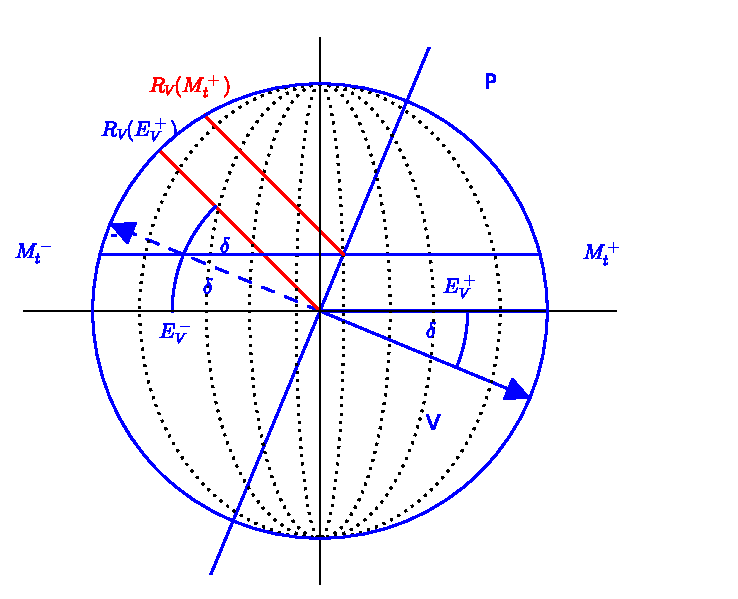
\includegraphics[width=.9\linewidth]{./reflection.pdf}
\caption{Reflection in the $(\vertvec, \reflectionvector)$-plane showing the reflected equator, \(M_T\), \(\reflectionmap(M_t)\) and some geodesics through the north pole (dotted lines).}
\label{fig:reflection}
\end{figure}
\subsection{Star-shaped hypersurfaces and one-sided reflections}
\Theo{rem}{starshaped}{
Recall a nonempty set $S\in \S^{n+1}$ to be star-shaped around $e,$ if $\pm e\notin S$ and if every geodesic from $e$ to $-e$ hits $S$ at most once, i.e.,
$$\forall x\in E\cn \# \br{\mrm{Im}~\g_{x}\cap S}\leq 1.$$
In this case we have a well-defined graph function of $S,$
\begin{align*}f_{S}\cn \pr{S}&\ra \br{-\fr{\pi}{2},\fr{\pi}{2}}\\
            \s&\mt \arcsin\inpr{x_{\s}}{e}, \end{align*}
where $x_{\s}$ is the unique preimage of $\s$ in $S$ under the projection $\pr.$ We obtain a parametrization of the set $S$ via the correspondence
$$x_{\s}=(\s,f_{S}(\s)).$$
}
\Theo{defn}{ReflectsAbove}{
Let $S,~T$ be two star-shaped sets around $e$ with the corresponding functions $f_{S}$ and $f_{T}.$

(i)~We say that \it{S lies above T}, denoted by $S\geq T,$ if
$$\forall \s\in \pr{S}\cap\pr{T}\cn f_{S}(\s)\geq f_{T}(\s).$$
(ii)~~Let $V\in \R^{n+2}$ and suppose $R_{V}(S)$ and $T$ are star-shaped around $e.$ We say that \it{S one-sided reflects above T}, if
$$R_{V}(S^{+}_{V})\geq T^{-}_{V}.$$

}
\Theo{lemma}{Starshaped Reflection}{
Let $V\in\S^{n+1}$ and $0\leq\d\leq\d_{0}<\fr{\pi}{4}.$ Then

(i)~$R_{V}(E)$ is star-shaped around $e.$

(ii)~There exists a constant $c=c(\d_{0})>0,$ such that for any closed and convex hypersurface $M\sub\S^{n+1}$ satisfying
$$|f_{M}|\leq c,$$
the reflection $R_{V}(M)$ is star-shaped around $e.$
}

\pf{
(i)~Since $R_{V}(E)$ is also an equator, the only way not to be star-shaped around $e$ would be
$e\in R_{V}(E). $
But then, letting $e=R_{V}(x)$ with $x\in E,$
$$1=\inpr{R_V(x)}{e }=2\sin\delta_V\inpr{x}{V}\leq 2\sin\delta_V\cos\d_V,$$
which is impossible in the given range of $\d_{V}.$

(ii)~The distance from $e$ to $R_{V}(E)$ only depends on $\d_{V}$; therefore, for a sufficiently small graph function $f_{M}$ we also obtain $e\notin R_{V}(M).$ Since every convex hypersurface of the sphere is star-shaped with respect to any interior (and exterior) point, the claim follows.
}
It is easily seen that the equator $E$ one-sided reflects above itself, if $0<\d_{V}<\fr{\pi}{4}.$ Now we show that this is also true for any convex hypersurface $M$ with controlled curvature, which is $C^{1}$-close to $E$ (the reason for these strong assumptions is the trouble that arises at the reflection plane $V^{\perp},$ at which $M$ has the same height as its reflection). 
% To this aim, we start with the following observation.


% Let \(x \in M^+\), \(z = R(x) = x - 2\inpr{x}{V} V\). Let us also write \(x = (\tilde{x}, x^{n+2})\) with \(\tilde{x} \in \R^{n+1}\). Orthogonal projection onto \(\{x^{n+2} = 0\}\) is then given by \(\pi (x) = \tilde{x} = x - \inpr{x}{e} e\). Because the plane spanned by \(e\) and \(\tilde{x}\) contains \(x\) we find that
% \[
% \pr (x) = \frac{\tilde{x}}{|\tilde{x}|}.
% \]

% Now for \(x \notin P\), we have
% \[
% V = \frac{1}{2\inpr{x}{V}} (x - z)
% \]
% lies in the plane spanned by \(x\) and \(z\). Therefore, \(\tilde V = \pi(V)\) lies in the plane \(Q\) spanned by \(\tilde{x}\) and \(\tilde{z}\). But \(\pr(x) = \tilde{x}/|\tilde{x}|\) and likewise for \(z\), hence \(Q\) is the plane spanned by \(\pr(x)\) and \(\pr(z)\).

% Let \(C\) be the geodesic joining \(\pr(x)\) to \(\pr(z)\). This is the intersection of the plane \(Q\) with the sphere which contains \(\tilde{V}\). Now let \(y\in P\cap C\). Then \(y \in Q\) and \(\tilde{V} \in Q\). But \(\tilde{V}\) is tangent to the sphere at \(y\):
% \[
% \langle \tilde{V},y \rangle = \inpr{V - \inpr{V}{e}e}{y} = \inpr{V}{y} - \inpr{V}{e} \inpr{e}{y} = 0
% \]
% since \(y \in P \Rightarrow \inpr{y}{V} = 0\) and \(y \in E \Rightarrow \inpr{y}{e} = 0\).

% So we have \(C = Q \cap \S^{n+1}\) with \(Q\) spanned by \(y\) and \(\tilde{V}\) with \(y\perp \S^{n+1}\) and \(\tilde{V} \in T_y \S^{n+1}\). Thus \(\tilde{V}\) is tangent to \(C\) at \(y\).

% The normal to the plane \(P\) is \(V\) and so at \(y\),
% \[
% \langle \tilde{V},V \rangle= \inpr{V - \inpr{V}{e}e}{V} = \inpr{V}{V} - \inpr{V}{e}^2 = 1 - \sin^2{\delta} = \cos^2(\delta)
% \]
% is independent of \(x\). Therefore, we have a lower bound on the angle $C$ makes with $P$, independent of the choice $x\in M^{+}.$
\Theo{prop}{ReflectedM}{
For all $V\in\S^{n+1}$ with $0<\d_{1}\leq\d_{V}\leq \d_{0}<\fr{\pi}{4}$ and all $\Lambda>0$ there exists $\a=\a(\d_{0},\d_{1},\L)>0,$ such that all closed and convex hypersurfaces with $e\notin M,$
$$0\leq f_{M},\quad |f_{M}|_{C^{1}(\mathbb{S}^n)}\leq\a\quad\text{and}\quad H\leq \L$$
one-sided reflect above themselves.
}
\pf{Suppose on the contrary that there exist a $V\in\S^{n+1}$ with $0<\d_{V}\leq \d_{0},$ $\Lambda>0$ and a sequence of hypersurfaces $M_{n}$ with
\eq{\label{eq:Sequ}0\leq f_{M},\quad |f_{M_{n}}|_{C^{1}(\mathbb{S}^n)}\leq \fr 1n,\quad H_{n}\leq \L,}
such that $M_{n}$ do not one-sided reflect above themselves (here, $H_n$ denotes the mean curvature of $M_n$); that is, $R_{V}(M_{n}^{+})$ does not lie above $M_{n}^{-}$ (from now on we suppress the subscript $V$ for better readability). Therefore, by \cref{ReflectsAbove}, there exist sequences
$$x_{n}\in M_{n}^{+},\quad y_{n}\in \mrm{Im}~\g_{R(x_{n})}\cap M_{n}^{-},$$
such that
\begin{equation}\label{eq: cont}
\inpr{R(x_{n})}{e}<\inpr{y_{n}}{e}.
\end{equation}
Thus
\eq{\inpr{x_{n}}{e}&=\inpr{R(R(x_{n}))}{e}\\
                &=\inpr{R(x_{n})}{e}-2\inpr{R(x_{n})}{V}\inpr{V}{e}\\
                &=\inpr{R(x_{n})}{e}+2\sin \d\inpr{R(x_{n})}{V}.}
Therefore, in view of (\ref{eq: cont}) this yields
\[0=\lim_{n\ra\8}\inpr{x_{n}}{e}= \lim_{n\ra\8}\br{2\sin\d\inpr{R(x_{n})}{V}}.\]
Thus, we may assume that
$$\inpr{x_{n}}{V}\ra0,\quad x_{n}\ra x\in V^{\perp}\cap E.$$
Hence we also obtain
\eq{\label{Conv}R(x_{n})\ra x,\quad y_{n}\ra x,\quad \pr(x_n)\ra x\quad\text{and}\quad \pr(y_n)\ra x.}
Denote by $C_{n}$ the unique great circle in $E$ containing $\pr(x_{n})$ and $\pr(y_{n})=\pr(R(x_n))$. Note that $C_n$ is well-defined for $n$ large enough; that is, $\pr(x_n)\ne \pr(R(x_n)),$ since $M_n$ is star-shaped and $x_n$ and $y_n$ are close to each other. 

The circles $C_n$ arise as the intersections of $E$ with some $2$-planes $Q_n;$ $C_n=E\cap Q_n.$ Consider the projection of $x_n$ to $E$,
$\pr(x_n)=\fr{\~x_n}{|\~x_n|},$
where $\~x_n=x_n-\inpr{x_n}{e}e.$ We have
\[\~x_n,~\widetilde{R(x_n)}\in Q_n.\]
Moreover, since
\[V=\fr{1}{2\inpr{x_n}{V}}\br{x_n-R(x_n)},\]
we also have $\~V\in Q_n$ and thus $\pr(V)\in Q_n$ for all $n.$ Along $V^{\perp} \cap E$, since $\pr(V)$ is a linear combination of $V$ and $e$, it is tangent to $\S^{n+1}$ and hence $\pr(V)$ is tangent to $C_n$ at $C_n \cap V^{\perp}$.

Now $C_n \cap V^{\perp}$ consists of two antipodal points. Let $p_n \in C_n \cap V^{\perp}$ be the closest point to $x_n$. Since $x_n \to x \in V^{\perp} \cap E$, $p_n$ is well defined for $n$ large enough.

From the circles $C_n$ we will construct curves $\l_n$ and $\mu_n$ in $M_n$ and $R(M_n)$ respectively. The equator $E$ is diffeomorphic to $M_n$ via the map
\eq{X_n\cn E&\ra M_n\\
		\zeta&\mt \cos\br{f_{M_n}}\zeta+\sin\br{f_{M_n}}e.}
Define
\eq{\label{lambda} \l_n=X_n|_{C_n}.}
Parameterize $C_n$ by arc length such that for $\t_1^n<0<\t_2^n$,
\[\l_n(\t_1^n)=x_n,\quad \l_n(0)\in V^{\perp}\quad~\text{and}\quad \l_n(\t_2^n)=y_n,\]
which is equivalent to 
\[C_n(\t^n_1)=\pr(x_n)\quad\text{and}\quad C_n(\t^n_2)=\pr(y_n).\]
Then
\[\l_n'(\t)=DX_n(C_n(\t))\cdot C_n'(\t).\]
In view of \eqref{eq:Sequ}, the differential of $X_n$ converges to the identity and hence
\eq{\label{lambdaConv}\sup_{\t}|\l_n'(\t)-C_n'(\t)|\ra 0.}
Since $R$ is an isometry of $\S^{n+1}$, the map
\[Y_n=R\circ X_n\cn E\ra R(M_n)\]
is a diffeomorphism as well. 

Now define the curves $\mu_n$ in $R(M_n)$ by
\[\mu_n(\t)=Y_n\circ C_n(\t^n_2+\t^n_1-\t).\]
Then
\[\mu_n(\t^n_2)=R(x_n).\]
We will obtain a contradiction to \eqref{eq: cont} by proving positivity of the functions
\[\xi_n=\inpr{\mu_n}{e}-\inpr{\l_n}{e}\]
on an interval of length bounded below.
In fact, we have a the Taylor expansion with remainder term, namely
\eq{\xi_n(\t)&=\xi_n(0)+\xi_n'(0)\t+\xi_n''(\t_n)\t^2,\quad \t_n\in (-\pi,\pi).}
Now
\[\xi_n(0)=\inpr{R\circ\l_n(\t^n_1+\t^n_2)}{e}-\inpr{\l_n(0)}{e}\ra 0~\text{as}~ n\ra\8,\]
since $|\pr(x_n)-\pr(y_n)|\ra 0.$
Furthermore, since $DR=\mrm{Id}-2V\cdot V^{T},$ we obtain
\eq{\xi_n'(0)&=\inpr{\fr{d}{d\t}R\circ\l_n(\t^n_1+\t^n_2-\t)}{e}_{|\t=0}-\inpr{\l_n'(0)}{e}\\
		&=-\inpr{\l_n'(\t^n_1+\t^n_2)}{e}+2\inpr{\inpr{V}{\l_n'(\t^n_1+\t^n_2)}V}{e}-\inpr{\l_n'(0)}{e}.}
 The first and the last term in this equality both converge to zero. The middle term is uniformly positive. To see this, note that
 from \eqref{Conv} we obtain that $\t_{p_n}$ converges to zero, where $\t_{p_n}$ is defined by the requirement $C_n(\t_{p_n})=p_n.$ We have
\eq{\label{slope}|\l_n'(\t^n_1+\t^n_2)-C_n'(\t_{p_n})|&\leq |\l_n'(\t^n_1+\t^n_2)-C_n'(\t^n_1+\t^n_2)|\\
				&\hp{=}+|C_n'(\t^n_1+\t^n_2)-C_n'(0)|+|C_n'(0)-C_n'(\t_{p_n})|,}
which converges to zero due to \eqref{lambdaConv}. Since $C_n'(\t_{p_n})$ is either $\pr(V)$ or $-\pr(V),$ independently of $n,$ we obtain
\eq{\l_n'(\t^n_1+\t^n_2)\ra -\pr(V).}
for otherwise we had
\[\inpr{\l_n'(0)}{V}=\inpr{\l_n'(0)-\l_n'(\t^n_1+\t^n_2)}{V}+\inpr{\l_n'(\t^n_1+\t^n_2)}{V}\ra \inpr{\pr(V)}{V}>0,\]
which is impossible due to the choice of $\t^n_1$ and $\t^n_2.$ This implies that $\xi_n'(0)$ is uniformly positive. 

Taking into account  $|\xi''_{n}(\t_{n})|$ is uniformly bounded by a constant $c>0$ (in view of our assumption on the mean curvature) $\xi_n$ is bounded below by $c_{\delta}/2$ on a uniform interval $[0,c_{\delta}/2c]$. Since for $n$ large enough, $\t_{2}^{n}$ becomes as small as desired and we have a contradiction in view of (\ref{eq: cont}).
}
\subsection{Reflecting quasi-ancient curvature flows}
The final aim of this section is to show that for a solution of a curvature flow defined on an interval $(-T_{S},0),$ which converges backwards in time to $E$ in $C^{1}$ and has bounded curvature, the flow hypersurfaces are invariant under reflection about every hyperplane $V^{\perp}$ with $V\in E.$ Hence we somehow need to let $\d$ go to zero in the preceding proposition. Until now we only obtained that for a given $\d>0,$ all flow hypersurfaces in an interval $(-T_{S},T_{\d})$ one-sided reflect above themselves. Hence, we can not still deduce that any flow hypersurface has this property for $\d=0.$ To get rid of the dependence on $\d$ in the interval $(-T_{S},T_{\d})$, we will use the parabolic maximum principle.
\Theo{lemma}{MPReflection}{
Let the closed and convex hypersurfaces $M_{t},$ $-T_{S}<t<0,$ satisfy the parabolic curvature flow equation
\[\dot{x}=-F(\cW)\nu\]
in $\S^{n+1}$ and suppose
\[M_{t}\ra E,\quad t\ra -T_{S},\]
in the sense that $e$ lies in the enclosed convex bodies by $M_{t}$ for sufficiently small $t$ and the graph functions satisfy
\[|f_{M_{t}}|_{C^{1}(E)}\ra 0,\quad t\ra -T_{S}.\]
 Furthermore, suppose
 \[\limsup_{t\ra -T_{S}}H_{M_{t}}\leq\L<\8.\]
 Then there exists $T>-T_{S},$ such that for all $V\in \S^{n+1}$ satisfying
 \[0<\d_{V}\leq \fr{\pi}{8},\]
 $M_{t}$ one-sided reflects above itself for all $t\in (-T_{S},T).$
 }

\pf{
By \cref{Starshaped Reflection} and the $C^{1}$-convergence of $M_{t}$ we obtain $T>-T_{S},$ such that $M_{t}$ and $R_{V}(M_{t})$ are star-shaped around $e$ for all $t\in (-T_{S},T).$ We show that this $T$ already has the desired property. By \cref{ReflectedM}, we know that for a given $V\in \S^{n+1}$ with (suppressing the subscript $V$ again)
\[0<\d\leq \fr{\pi}{8},\]
 there exists $\~T_{\d}>-T_{S},$ such that $M_{t}$ one-sided reflects above itself for all $t\in (-T_{S},\~T_{\d}).$ Pick a $-T_{S}<T_{\d}<\~T_{\d}$ and define the domain
\[\O=\bigcup_{t\in(T_{\d},T)}\{t\}\times \pr(M_{t}^{-})\sub (-T_{S},T)\times E.\]
Recall from \eqref{eq:GraphCurvFlow} that the time dependent graph functions of the $M_{t}$ satisfy
\[\label{FullyNonlinear}\fr{\del}{\del t}w=-F\br{\fr{\vt'}{v\vt}\d^{i}_{j}+\fr{\vt'}{v^{3}\vt^{3}}\nabla^{i}w\nabla_{j}w-\fr{g^{ik}}{v}\nabla^{2}_{kj}w}v,\]
where $\vt=\vt\br{w}=\sin\br{w},$ $v^2=1+\vt^{-2}|\nabla w|^2$
and the connection and the norm $|\cdot|$ are those belonging to the spherical metric $\s_{ij}.$ Since the Weingarten operator is invariant under ambient diffeomorphisms, the reflected hypersurfaces $R_{V}(M_{t})$ with the corresponding graph functions $u$ satisfy the same curvature flow equation.

If the claim of the lemma were false, then there existed a time $t\in (T_{\d},T)$ and a point $x\in \pr(M_{t}^{-}),$ such that
\[\label{MPReflection1} u(x,t)>w(x,t).\]
Formally we would like to apply the parabolic maximum principle to conclude that $u$ must remain below $w,$ since this is the case at the initial time $T_\d$ and also at the boundaries $\del\br{\pr(M_t^{-})}\sub V^{\perp}.$ However, in this situation the application of the standard comparison principles to equations of the form
\[\dot{w}=\Phi(x,w,\nabla w,\nabla^2w)\]
is not straightforward, due to the restriction that $F$ is generally only defined on positive definite endomorphisms. In the following we make sure that we still get a contradiction to \eqref{MPReflection1}.


A slight rewriting of the second fundamental form of $M_t$ described by the graph function $u$ yields
\eq{h^i_j&=\fr{\vt'}{\sqrt{\vt^2+|\nabla u|^2}}\d^i_j+\fr{\vt'}{\br{\vt^2+|\nabla u|^2}^{\fr 32}}\nabla^iu\nabla_ju-\fr{\vt g^{ik}}{\sqrt{\vt^2+|\nabla u|^2}}\nabla^2_{kj}u\\
        &=\fr{\vt g^{ik}}{\sqrt{\vt^2+|\nabla u|^2}}\br{\fr{\vt'}{\vt}g_{kj}+\fr{\vt'}{\vt\br{\vt^2+|\nabla u|^2}}g_{km}\s^{mr}u_ru_j-\nabla^2_{kj}u}\\ 
        &\equiv \fr{\vt(u)g^{ik}}{\sqrt{\vt^2(u)+|\nabla u|^2}}A_{kj}(x,u,u,\nabla u,\nabla^2u),}
 where $\vt=\vt(u)$ and we set
 $$A_{kj}(x,z,u,p,r)=\fr{\vt'(z)}{\vt(z)}g_{kj}(u)+\fr{\vt'(z)}{\vt(z)\br{\vt^2(z)+|p|^2}}g_{km}(u)\s^{mr}p_rp_j-r_{kj}.$$
 Here the dependence on $x$ is hidden in $\s^{mr}$ and we artificially introduced $z$ in the argument in order to distinguish increasing behavior from decreasing behavior in $u.$ Observe that
 $$\fr{\del A_{kj}}{\del z}\br{x,z,u,\nabla u,\nabla^2u}<0\quad\text{on}~ z\in(0,u(x,t))$$
 in the sense of bilinear forms, whenever $u$ describes a strictly convex hypersurface. To see this, use that $\cot(z)$ is decreasing in $z.$
 
Also write
$$h^i_j(x,z,u,p,r)=\fr{\vt(z)g^{ik}(z)}{\sqrt{\vt^2(z)+|p|}}A_{kj}(x,z,u,p,r).$$
Hence, if $u$ graphs a convex hypersurface, we obtain that
$$\forall~ 0<z\leq u(x,t)\cn\quad h^i_j(x,z,u(x,t),\nabla u(x,t),\nabla^2u(x,t))>0$$
 and thus $h^i_j$ lies in the domain of $F.$ Write
  $$\Phi(x,z,u,p,r)=-F(h^i_j(x,z,u,p,r))\sqrt{1+\vt^{-2}(z)|p|^2}.$$
Now, by our assumption 
 $$0<u(x,t)-w(x,t)=\max_{\-\O}(u-w),$$
 at $(t,x)$, and we have $\dot{u}\geq \dot{w},$ $\nabla u=\nabla w$ and $\nabla^2u\leq \nabla^2w.$ Define 
 $$\~u=ue^{-\l t},\quad \~w=we^{-\l t},$$
 where $\l>0$ is determined by the requirement that
$$-\fr{\del\Phi}{\del z}(x,t,z,u(x,t),\nabla u(x,t),\nabla^2 u(x,t))+\l>0\quad\forall~ 0<z\leq u,
$$
 which is possible due to the smoothness of $\Phi$ on the given compact interval. We find at $(x,t)$ that
\eq{\br{\dot{u}-\Phi(x,u,u,\nabla u,\nabla^2u)}e^{-\l t}&=\dot{\~u}-\Phi(x,u,u,\nabla u,\nabla^2 u)e^{-\l t}+\l\~u\\
        &\geq \dot{\~u}-\Phi(x,w,u,\nabla u,\nabla^2 u)e^{-\l t}+\l\~w \\
        &> \dot{\~w}-\Phi(x,w,w,\nabla w,\nabla^2w)e^{-\l t}+\l\~w\\
        &=\br{\dot{w}-\Phi(x,w,w,\nabla w,\nabla^2 w}e^{-\l t},
    }    
 a contradiction, since both sides are zero in view of the flow equation.
}
\begin{thm}
\label{thm:classification}
Let \(M_t\) be a convex, embedded (quasi-)ancient solution of any (uniform whenever on uniformly convex hypersurfaces) parabolic equation on \(\S^{n+1}\) such that \(M_t \to E\) in \(C^1\) as \(t \to -T_S\) with uniform \(C^2\) bounds. Then \(M_t\) is a family of shrinking geodesic spheres emanating from the equator \(E\) at \(t=-T_S\).
\end{thm}
\begin{proof}
From \cref{MPReflection} we have \(\reflectionmap(\reflectionset{(M_t)}^+) \geq \reflectionset{(M_t)}^-\) everywhere for all \(t \in (-T_S, -T)\) and any \(\reflectionangle \in (0,\reflectionangle_0)\). By continuity therefore, sending \(\reflectionangle \to 0\) we have \(\reflectionmap(\reflectionset{(M_t)}^+) \geq \reflectionset{(M_t)}^-\) for all \(t \in (-T_S, -T)\)  and any \(\reflectionvector\) satisfying \(\ip{\reflectionvector}{\vertvec} = 0\).

Now, we need some simple properties of $\reflectionmap[\reflectionvector]$ following from the fact that $\ip{\reflectionvector}{\vertvec} = 0$:
\begin{itemize}
\item $\reflectionmap^2 = \id$,
\item $S \geq T \Rightarrow \reflectionmap(S) \geq  \reflectionmap(T)$,
\item $\reflectionmap = \reflectionmap[-\reflectionvector]$, and
\item $\reflectionset{S}^{\pm} = \reflectionset[-\reflectionvector]{S}^{\mp}$.
\end{itemize}
Thus we obtain
\begin{align*}
\reflectionset{(M_t)}^+ &= \reflectionmap(\reflectionmap(\reflectionset{(M_t)}^+)) \geq \reflectionmap(\reflectionset{(M_t)}^-) \\
&= R_{-V}((M_t)^+_{-V}) \geq \reflectionset[-\reflectionvector]{(M_t)}^-\\
&= \reflectionset{(M_t)}^+.
\end{align*}
So we must have equality all the way through and hence the middle line implies
\[
R_{-V}((M_t)^+_{-V}) = \reflectionset[-\reflectionvector]{(M_t)}^-
\]
for any $\reflectionvector$.

Therefore, \(M_t\) is invariant under \(\reflectionmap\) for any \(\reflectionvector\) satisfying \(\ip{\reflectionvector}{\vertvec} = 0\) and hence is a geodesic sphere for every \(t \in (-T_S, T)\) and by uniqueness of solutions, is a geodesic sphere for every \(t \in (-T_S, 0)\).
\end{proof}

\bibliographystyle{amsplain}
\bibliography{Bibliography.bib}


\end{document}
